\chapter{Sentence Reader}\label{chap:sentreader}

In Chapter \ref{chap:viewer}, we have talked about Pāli document viewers that are equipped with tools facilitating enjoyable readings. For a study of Pāli text, familiarity with those viewers is sufficient in most cases. I myself, when reading a scripture, use those viewers most of the time.

To help new students, as a developer, I have come up with the idea of \emph{Sentence Reader} since the release of \textsc{Pāli\,Platform\,2}. The basic concept is simple: ``It would be nice if we can have definitions of all words in the passage we are reading.'' Unfortunately for beginners, apart from that basic function, now the Reader (together with the Manager, explained later) has grown into a sophisticated device for manipulating Pāli sentences. That makes the tool so complex that it scares away new users.

To prevent pushing this toolset into marginal state, destined to be removed in the future, I have exerted an effort to improve the related tools, making them work properly with the recent release of \textsc{Pāli\,Platform}. Another factor that makes the Reader usable is the integration of the DPD. With this massive dictionary, now we can read a passage a lot easier than before.

\section{Basic operations}

Before we go into formidable details, let us be familiar with the basic functions. To invoke a Sentence Reader, you can either use menu Sentence > {\faSix \symbol{"F518}} Sentence Reader or open it with a text portion in viewers (see Figure \ref{fig:sentreader-fromviewer}) or Text Editor. In case of opening a blank Reader, you can put some text in by copying it from somewhere and pasting it here.

\boxnote{Apart from launching Sentence Reader from text viewers, you can do likewise in Text Editor by selecting a portion of text, if you do not use the whole file, then choose menu Tools > Read text.}

\begin{figure}[!hbt]
\centering
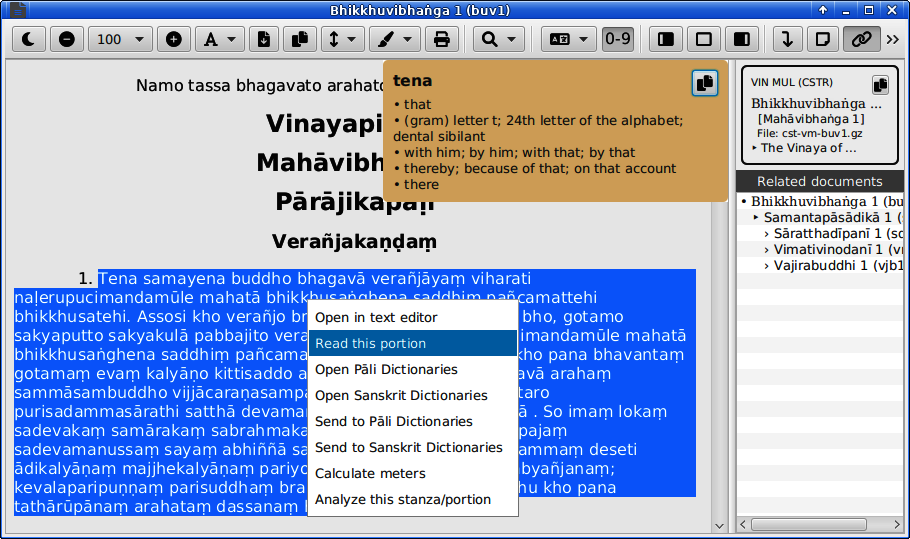
\includegraphics[width=0.9\linewidth]{images/sentreader-fromviewer.png}\\
\caption{Opening Sentence Reader from a viewer}
\label{fig:sentreader-fromviewer}
\end{figure}

As shown in the picture, when you select a portion of text and do a right-click, you have an option from the context menu to open the portion in Sentence Reader. Once you select the menu, a Reader window will be opened with the text selected. The passage will be broken down to sentences, and you will see the first sentence in simple mode at first (see Figure \ref{fig:sentreader-simpleview}).

\begin{figure}[!hbt]
\centering
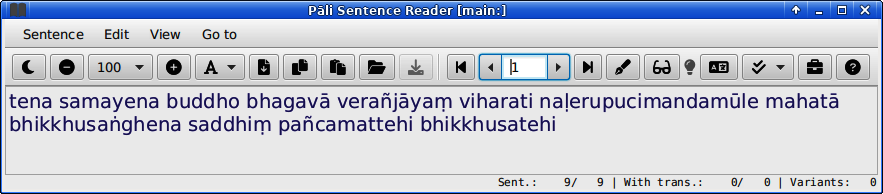
\includegraphics[width=0.9\linewidth]{images/sentreader-simpleview.png}\\
\caption{Sentence Reader in simple view}
\label{fig:sentreader-simpleview}
\end{figure}

The next thing you should do is clicking {\faSix \symbol{"F530}} button (or press \texttt{Ctrl-I}) to enable detailed view. If you have DPD installed, you will see the result similar to Figure \ref{fig:sentreader-detailview}. The text portion taken in the example is the first paragraph of the Vinaya.

For the basic usage, this seems to be enough in most cases when you take a passage to read. You just learn how to navigate the sentences back and forth using buttons, menu, or shortcuts provided. An option you should be aware of is the DPD integration (see Figure \ref{fig:dpd-integration} on page \pageref{fig:dpd-integration}). If this option is turned off, the lookup will use the program's facilities instead, such as CPED, pronoun list, etc.

\begin{figure}[!hbt]
\centering
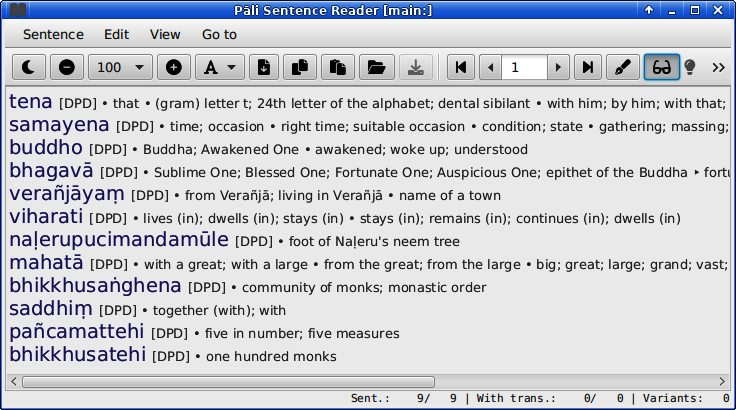
\includegraphics[width=0.9\linewidth]{images/sentreader-detailview.png}\\
\caption{Sentence Reader in detailed view}
\label{fig:sentreader-detailview}
\end{figure}

Another feature you may find useful is the ability to save the sentences as a sequence (explained below). You can do this by selecting menu Sentence > Save this sequence, then giving a name to the sequence and choosing a directory (the default directory is `\texttt{main}'). Then you can open the sequence afterward by selecting menu Sentence > {\faSix \symbol{"F07C}} Open a sequence (\texttt{Ctrl-O}), or clicking {\faSix \symbol{"F07C}} button.

\boxnote{To add text to Sentence Reader after copying it from somewhere, simply press \texttt{Ctrl-V}\\
\hspace{5mm}\bullet\ or click {\faSix \symbol{"F0EA}} button\\
\hspace{5mm}\bullet\ or use menu Sentence > {\faSix \symbol{"F0EA}} Paste text
}

\section{Concepts explained}

To get the best benefits from the Reader, you have to know the concepts behind the design. This can be difficult for non-technical users, but it is worth knowing, at least the meaning of key terms.

\subsection{Sentence and sequence}

The unit counted as a sentence does not like a sentence (a meaningful group of words strung together) in any language, even if it looks like that. A sentence here is a portion of text that can be cut apart by delimiters. Knowing the possible delimiters is helpful for understanding the tool's behaviors. A number of delimiters are recognized so far as follows:

\paragraph{Capitalization} Using a capitalized term as a sentence marker is applicable to documents that are formatted with capitalization. CSTR is a notable one.\footnote{As I have noted elsewhere, capitalization in CSTR is the remnants of the former CSCD, Roman edition. It is not perfect, or it could be better.}

\paragraph{Bars (|\,‖)} Vertical bars and double bars are used as sentence ending in CST4 texts, converted by Least Contamination method (see Section \ref{sect:cst-xml} on page \pageref{sect:cst-xml}).

\paragraph{Dot (.)} A general fallback of sentence delimiters is periods. If a document uses no capitalization or bars, this can be helpful. But it can cause a confusion when other forms of dot are also used, such as after abbreviations.

\paragraph{Colon (:)} I found that documents in the BJT collection use colons in this way, like English. Users of this corpus should be aware of this.

\paragraph{Semicolon (;)} This token is often used with verses. Reading a stanza with this delimiter enabled can be helpful.

\paragraph{Dashes (--\,---)} This is optional. You may want to treat dashes, both short dash (U+2013, called n-dash) and long dash (U+2014, called m-dash), as delimiters. Or, you may keep their presence in sentences.\footnote{When dashes are processed, all m-dashes are converted to n-dashes.} Note that only independent dashes (surrounded by spaces) are treated in this way, not dashes connecting words. And the minus sign or hyphen (-) is not counted as a dash. This will be removed when the text is processed.

\bigskip
All of these delimiters can be turned on or off in the Sentence tab of Settings window, shown in the lower part of Figure \ref{fig:settings-sentence}.

\begin{figure}[!hbt]
\centering
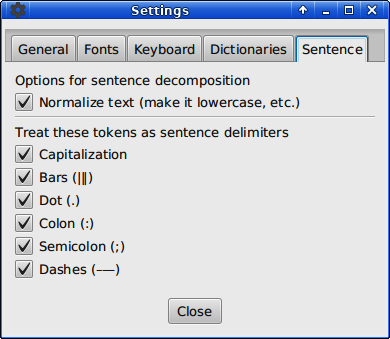
\includegraphics[width=0.7\linewidth]{images/settings-sentence.png}\\
\caption{Sentence tab of Settings}
\label{fig:settings-sentence}
\end{figure}

After sentences are broken down, each of them is processed further by tokenization to remove all symbols (except ? and !). The sentence can be normalized, or made lowercase, if this option is enabled (see the upper part of Figure \ref{fig:settings-sentence});

Once a sentence is identified, it will have two forms: \emph{text} and \emph{edit}. The \emph{text} is the string of words unique to the sentence, all symbols removed. This part is \emph{immutable} and used to generate sentence's identifier called \emph{hash}.\footnote{Hash is a string of hexadecimal numbers. It is calculated from its corresponding sentence (the \emph{text} part). Each sentence has its own hash. A collision of the same hash from different strings is possible but very unlikely. Technically, MD5 digest calculation is used here.}

The \emph{edit} form of a sentence is \emph{mutable} with some symbols retained, such as dashes, question marks, and exclamation marks. You can change this part in whatever way you like by enabling {\faSix \symbol{"F5AC}} button, but its identifier is still the same because its original version kept in the \emph{text} part is unchanged. Note that it is the edit form of a sentence that is shown in the display of the Reader. Once you severely ruin the edit, you can restore to the original by using the context menu (right-click).

The usefulness of having the \emph{edit} form is you can slightly change the sentence to ease the word lookup or experiment with some ideas. For example, you can break down a long compound by inserting hyphens (minus signs) in the word. Then you can see the definition of each part. DPD makes this unnecessary, but it can still be done.

Once a sentence is saved in a different folder which already contains the same hash (meaning the two sentence is identical), you will be asked to keep or overwrite the existing one. If the old instance is replaced, the new \emph{edit} of the sentence (also all variants of translation, explained below) is used instead.

One consequence of generating a sentence in this way is that it is \emph{reusable}. By the nature of Pāli text composition, many sentences are reused or repetitive in form. One sentence can appear in several contexts. In a way, we can call a highly frequent sentence as a \emph{stock sentence}.\footnote{This tool can open an opportunity to research on this topic, but you have to process a lot of sentences to see significance in their statistics.}

A sentence does not stand alone. It always sits together with other sentences. Here comes the concept of \emph{sequence}. It means a group of sentences strung together with a predefined order. If you copy a paragraph of text and paste it into the Reader, you get a sequence of that paragraph's sentences. This paragraph or sequence can be saved with its own name, and opened later. You may create a sequence from a bigger unit, like a section or even a book.\footnote{Up to now, only sentence and sequence have meaning in the Reader. The concept of \emph{section} (ordered sequences) and \emph{book} (ordered sections) are not implemented yet (not even in the plan).}

\subsection{Translation and variant}

What makes the tool complicated is the attempt to add translations to sentences. The infrastructure described so far and the data structure used make this possible. To open the translation pane, click {\faSix \symbol{"F1AB}} button, or hit \texttt{Ctrl-T}. If a sentence already has a translation, you can see the green light bulb. When opening the pane with all variants ({\faSix \symbol{"F069}} enabled), you can see something similar to Figure \ref{fig:sentreader-translations}.\footnote{This sequence was bundled with \textsc{Pāli\,Platform\,2}, now removed from the package. The sentences in this set are still valid to use, albeit a little outdated. You have to download its packed file manually at \url{github.com/bhaddacak/pp2-sentences} and unpack it to directory \texttt{data/sentences}.}

\begin{figure}[!hbt]
\centering
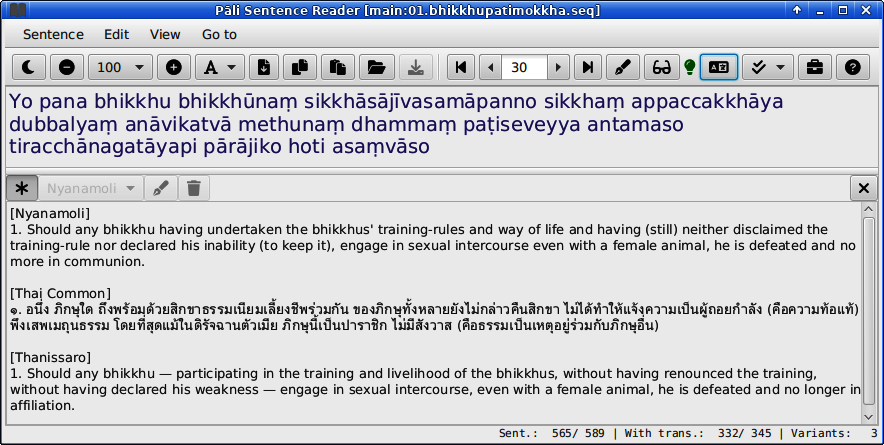
\includegraphics[width=0.9\linewidth]{images/sentreader-translations.png}\\
\caption{A sentence with translations}
\label{fig:sentreader-translations}
\end{figure}

Let us come to the term. A \emph{variant} is a variation of translation identified by its author or related information. One author can also be represented by several variants, or seen as versions. By the use of variants, we can add translations, including any native language\footnote{By native language, I mean the language or locale of the users recognized by their system. So, fonts for that language should be always available.}, as many as we need to a single sentence. This can demolish the illusion of one correct translation.

I will not go into every bit of how to use the tool. If you see that it might considerably help you in learning the language, you should take time to experiment by yourselves. Learning things the hard way always brings sustainable results.

However, the numbers summarized on status bar need some explanations. As shown in the picture, the status bar of that example is read as follows:

\begin{center}
\fbox{\ttfamily\small Sent.: 565/ 589 | With trans.: 332/ 345 | Variants: 3}
\end{center}

The first part tells us how many sentences in this sequence totally. The first number (565) is the count of distinct sentences, the second (589) the count of all sentences. The difference (589 - 565 = 24) tells us how many times the distinct sentences are repeated. If the difference is high, the passage is very repetitive, so to speak.

The middle part tells us how many sentences having translations. The first number (332) is for distinct sentences, the second (345) all of them. The last part shows the total number of variants (3). It tells us that there are three sources or authors of translations used in this sequence.

Another thing you should know is when you create a new sequence in a new directory and want to add a translation to its sentences, you need at least one variant to be present. If you have not created a variant for that directory yet in Sentence Manager (see Chapter \ref{chap:sentmanager}), the variant will be `Default'. When you create a new variant while the Reader is opened, you may have to update it by menu Sentence > Update variant list. For a massive addition of translations, using Sentence Manager is more convenient.

As you may note, by this model of implementation, sentences are separated from their contexts. We have the sentence pool in a directory. When we read a sequence, it picks its sentences, which may have translations embedded, from the pool. You may see this as a drawback because one sentence may need different translations in different contexts. However, this treatment is suitable for the repetitive nature of the Pāli text, I think.

\boxnote{To summarize:\\
\hspace{5mm}\bullet\ \textbf{Sentence} is a string of words, determined by selected delimiters.\\
\hspace{5mm}\bullet\ \textbf{Text} form of a sentence is regarded as original. It is immutable.\\
\hspace{5mm}\bullet\ \textbf{Edit} form of a sentence is mutable \emph{text}.\\
\hspace{5mm}\bullet\ \textbf{Hash} of a sentence is its identifier, computed from the \emph{text} part.\\
\hspace{5mm}\bullet\ \textbf{Sequence} is a list of sentences that has a fixed order.\\
\hspace{5mm}\bullet\ \textbf{Translation} is an additional data or explanation added to a sentence.\\
\hspace{5mm}\bullet\ \textbf{Variant} is a variation of translation.
}

\section{Grammatical options}

The meaning lookup of each word in a sentence is not the whole story. The tool is also armed with some grammatical aids, as shown in options provided under {\faSix \symbol{"F560}} menu button. 

One option worth talking about here is the reconstruction of \pali{iti}. In CST4 texts, for example, when \pali{iti} is marked out, for example, \pali{vilapi'nti}, the sandhi term will be tokenized into two words, i.e., \pali{vilapi} and \pali{nti}. When the option of \emph{Reconstruct\,iti} is turned on, we will get \pali{vilapiṃ} and \pali{iti} in the display (but the edit text is still intact).

Another example, \pali{passāmī'ti} yields \pali{passāmī} and \pali{iti}. And if the option of \emph{Shorten\,vowel\,before\,iti} is also turned on, \pali{passāmī} will become \pali{passāmi}.

That is what we expect when we learn in Pāli classes. But things do not go that easy. In some instances, shortening the vowel does not make the right word, and the program does not know that. So, you have to make a decision whether you should use the option or not. Either way is not perfect.

For the terms that seem to have \pali{iti} but it is not marked out, e.g., \pali{abhinandunti}, you can separate the \pali{ti} (or \pali{nti} in this case) manually by editting the sentence, hence \pali{abhinandun ti}.

Figure \ref{fig:sentreader-options} illustrates the points in the examples mentioned. It worth noting that when you insert independent double hyphens (minus signs), you will get a dash in the display as the picture shows.

\begin{figure}[!hbt]
\centering
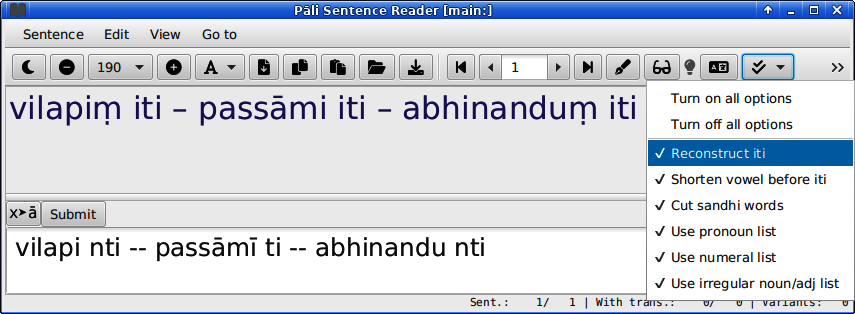
\includegraphics[width=0.9\linewidth]{images/sentreader-options.png}\\
\caption{Reconstructing iti as a grammatical option}
\label{fig:sentreader-options}
\end{figure}

The option of \emph{Cut\,sandhi\,words} can be helpful to new students. When this is turned on, the predefined table of sandhi words will be looked up and help cutting the words accordingly. For example, when the Reader sees \pali{nāhaṃ}, it will cut the word into \pali{na} and \pali{ahaṃ}.\footnote{This has nothing to do with the deconstructor of DPD because the deconstructor table is not used in the Reader.} Please try this yourselves.

Other options, i.e., the use of pronoun/numeral/irregular list, will be not active (even selected) when DPD is in use. These three tables precede the DPD, but they have some merits when DPD is not available.

Another option, not shown in the menu, is the custom dictionary. When DPD is not used, the custom dict will be looked up first, then CPED. You can edit this custom dict with the menu provided.\footnote{See menu Edit. You can do likewise with the sandhi list. Technically, the two files are in directory \texttt{data/rules} with their corresponding name. Note that there is no option to turn the custom dictionary off. You have to comment out the entries when you exclude words.}

\section{Concluding remarks}

Sentence Reader is a powerful learning tool. To gain the best out of it, you have to invest time and effort in learning the tool, as well as the concepts behind the design. To most users this is still overkill. But to developers, this can demonstrate the power of imagination and show potentials of yet more powerful learning tools to be developed in the future.

